\chapter{Background}
\section{Plant-microbe interactions}
The plant microbiome is made up of communities of microorganisms that inhabit the internal and external of plants, collectively forming a dynamic ecosystem that supports plant growth and pathogen protection. Rather than acting as completely isolated domains, the plant's two main spatial regions: the above-ground phyllosphere and the below-ground rhizosphere. Each encompasses both external (exosphere) and internal (endosphere) environments. The rhizosphere is the zone around plant roots, this zone is heavily enriched with organic materials from the plant and products from microbes and other organisms in this environment. 
As plants allocate up to 20\% of their photosynthetically derived carbon as exudates into the rhizosphere, the nutritional value of root released metabolites is high and therefore attracts soil microbes to the root (\cite{trivedi_plantmicrobiome_2020, hutsch_plant_2002}).
Members of a plant microbiota comprise beneficial, neutral, and pathogenic microorganisms, whose relative activity and balance determine whether microbiome function supports or undermines host health. Importantly, certain microbial traits manifest only within the context of a whole community and cannot be predicted from individual members alone (\cite{trivedi_plantmicrobiome_2020}).
\subsection{Metabolic interactions within microbial communities}
Metabolic interactions are driven by cross-feeding, antagonism and niche differentiation. A metabolic niche can be described as the set of genetically encoded metabolic functions that an organism needs to survive. Niche differentiation is the process by which competing species use the environment differently in a way that helps them to coexist. Antagonistic interactions are characterised by the secretion of specialised metabolites, which inhibit competitors or restrict their access to essential nutrients (\cite{wankhade_review_2025}). Cross-feeding describes interactions, where one microorganism consumes and utilises the metabolic byproducts or waste compounds secreted by another. Within such dynamics, certain community members can act as keystone species, playing an especially important role in stabilising their ecosystem. They exert a large number of (positive) interactions and their removal from the system significantly affects ecosystem productivity, nutrient cycling, and species richness (\cite{amit_top-down_2023, banerjee_keystone_2018}).
\subsection{Design and applications of synthetic communities}
Microbial communities compose a significant part of the rhizosphere. Elucidating the detailed mechanisms behind plant-microbe and microbe-microbe interactions however remains challenging, as the complex natural communities are difficult to analyse: Which members are actively participating in nutrient exchanges? Are all occurring rare species cultured? Which players perform key functions? (\cite{shayanthan_role_2022}). Some of these questions can be answered using Synthetic Communities (SynComs), which are composed of selected bacterial strains that together represent a simplified version of the microbiome while retaining functional traits. They are widely established as model systems for the analysis of performance, structure and stability of microbial communities. As the exact composition of the co-culture and the surrounding conditions are known, these defined systems reduce complexity while preserving key attributes of the natural community they represent (\cite{groskopf_synthetic_2014}). 
\subsubsection{Synthetic communities HvSC1 and HvSC2}
\cite{mahdi_low_2026} extensively cultured barley root endophytes across genetically distinct barley accessions, from which the SynComs investigated in this thesis were composed. Core strains were assembled to the core SynCom, HvSC1, its 29 members reflect taxonomic composition in the natural barley microbiome. The trait-prioritised SynCom, HvSC2, was assembled based on 26 strains previously associated with plant growth promotion or pathogen suppression and does not reflect natural co-occurrence (Fig. \ref{fig:taxonomic_distr}).
Experimental comparison of the two SynComs showed that microbial communities exhibiting little disruptive competition and low antagonism are favoured by host-associated environments. Beneficial microbiome function is promoted by balanced interspecies interactions rather than maximal antagonism and limited disruptive competition within a community. The conducted experiments contrasted the two communities in their antagonistic behaviour, stability and impact on plant growth: the core SynCom exhibited low antagonism and high stability, while guarding the host plant against fungal pathogens without reducing plant growth. Contrastingly, the trait-optimised SynCom was characterised by pervasive antagonism, competitive exclusion, community instability, and despite being composed of strains with predicted plant growth promoting traits, yielded loss of plant protective function and diminishing root growth (\cite{mahdi_low_2026}).

\begin{figure}[h]
  \centering
  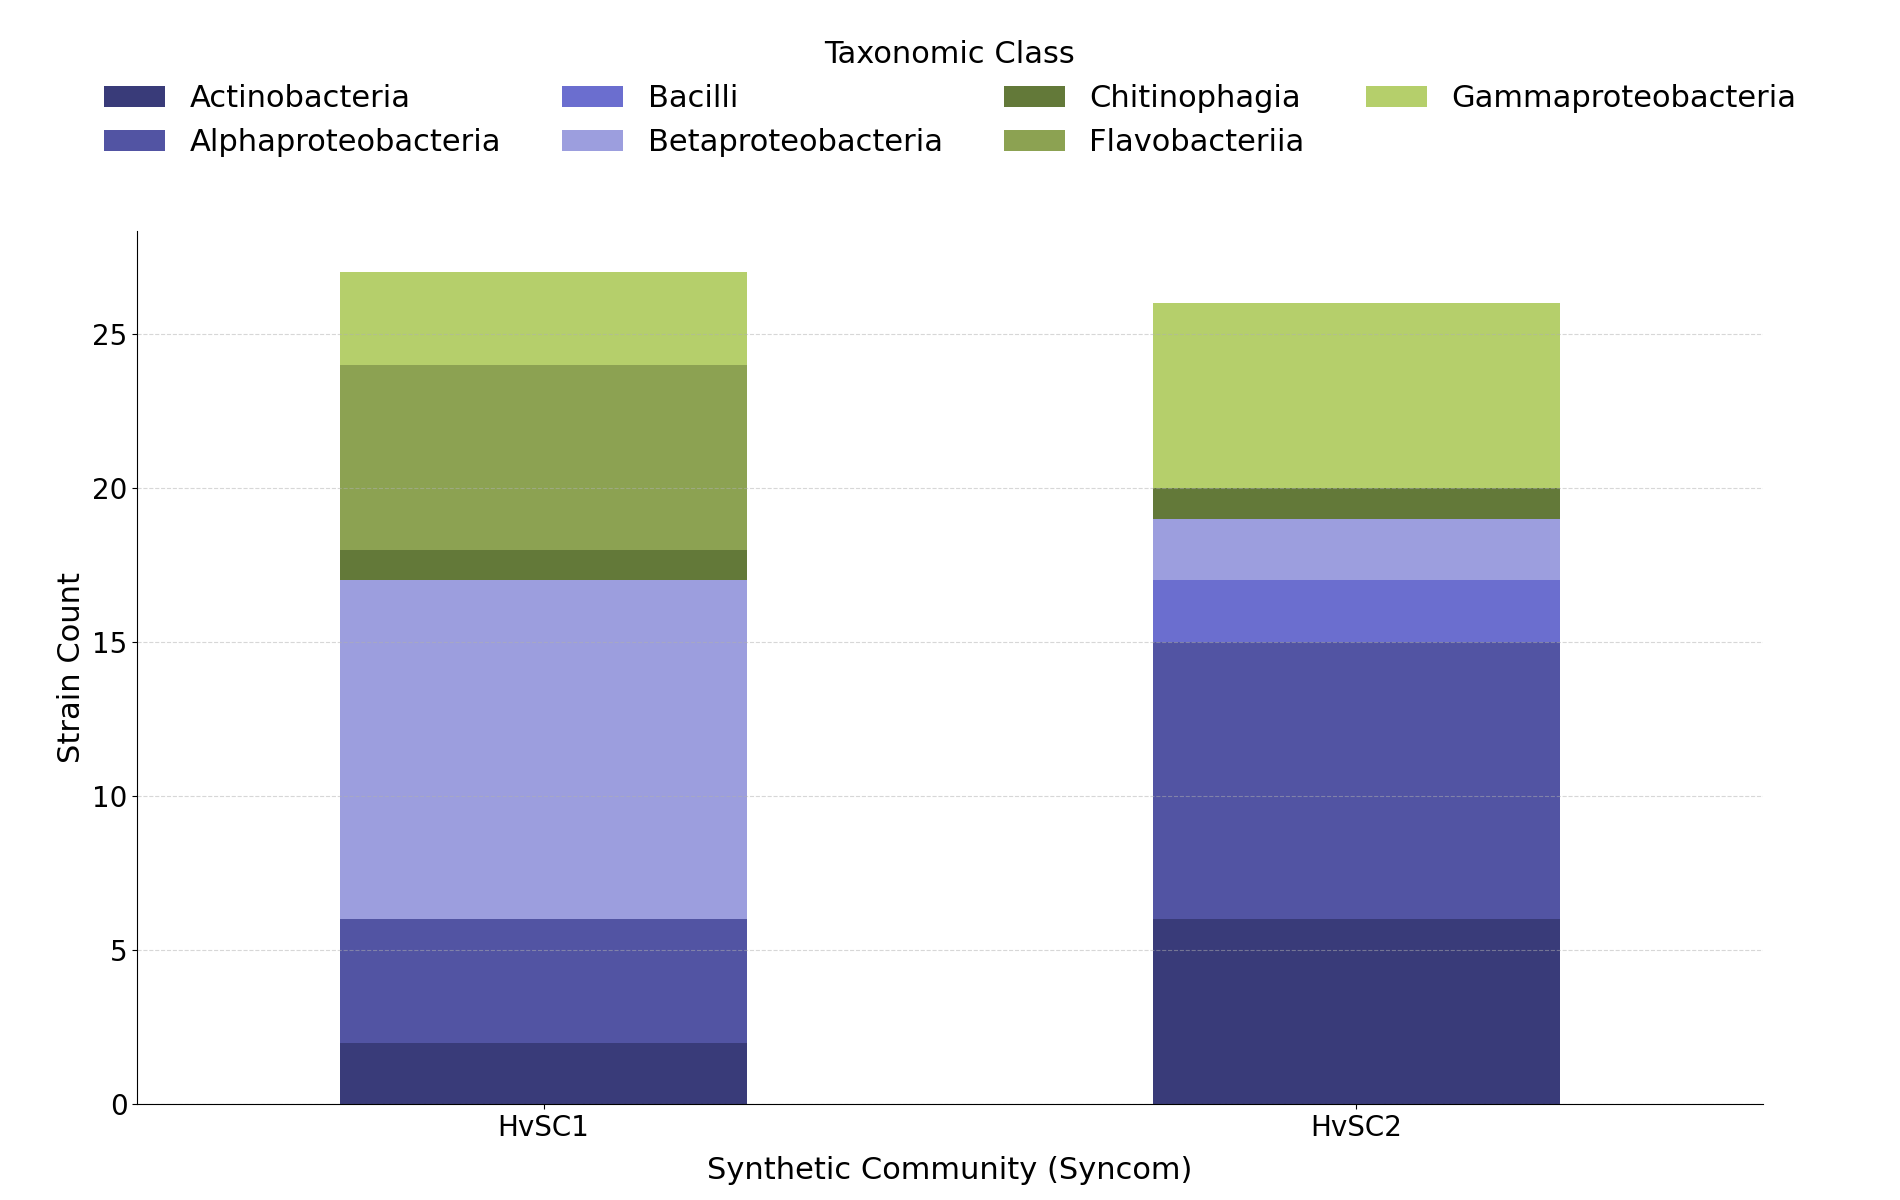
\includegraphics[width=1\textwidth]{fig/taxonomy_distr.png}
  \caption[Taxonomic class composition of the barley SynComs]{Taxonomic class composition of the barley SynComs. Stacked bar chart displaying the strain count across various taxonomic classes for two HvSC1 and HvSC2. Colors denote specific bacterial classes as indicated in the legend.}
  \label{fig:taxonomic_distr}
\end{figure}

\section{Genome-scale and constraint-based metabolic modelling}
\subsection{Metabolic network reconstruction}
Studying the complexity of metabolism in nature is often very challenging. Reconstructing metabolic networks into computational formats reduces complexity and can provide valuable insights into underlying structures.
Metabolic networks can be reconstructed in different approaches. Kinetic metabolic reconstruction is based on determining the appropriate reaction network followed by parameterising the rate laws with empirically based values, thereby allowing the simulation of dynamic behavior within a cell (\cite{cook_standardized_2026}). Stoichiometric based modelling is an alternative approach, which relies on metabolic steady states, meaning that the sum of all changes in metabolite concentrations $x$ over time is $0$ (\cite{orth_what_2010}). This approach requires less data and is therefore much more practical for genome-scale metabolic models and was employed in this thesis.
\\


Genome-scale metabolic models (GEMs) translate genomic information into mathematical formulations of metabolic networks. Such a metabolic network is represented as a stoichiometric matrix ($S$) of size $m  \times n $. Every row of this matrix represents one unique compound, every column a reaction, yielding $m$ metabolites and $n$ reactions. The entries of one column are the stoichiometric coefficients of the metabolite in this reaction. These are negative if the metabolite is consumed in the reaction and positive if this metabolite is produced in the reaction. A coefficient of zero means that the metabolite does not participate in the reaction. The flux through all the reactions of the system is represented by the vector $v$, with length $n$, the metabolite concentrations are represented by the vector $x$ with length $m$. Under the steady-state assumption, the system is described by $Sv = 0$. 
\\


One method to investigate these metabolic networks is constraint-based modelling (CBM), which can be used to analyse the solution space. A solution space is defined by all feasible phenotypic states, given a set of imposed constraints. These constraints arise from the relationship between the genotype of an organism, its environment and physico-chemical laws (\cite{bordbar_constraint-based_2014}). CBM scales to large-scale models, provides mechanistic understanding of molecular processes and does not require kinetic parameters, which are often hard to obtain. The strategy involves two major steps: first, constraining a biological system and then analysing the system to predict metabolic fluxes (Fig. \ref{fig:fbaworkflow}). 
\\


The constraining of a model usually modifies the metabolic reaction bounds and thereby defines the solution space. This can be achieved using various types of data, such as the uptake and secretion profiles of metabolites, or the expression levels of mRNA and proteins, to either setting the bounds of a reaction to zero if the corresponding protein is absent or scaling the bounds to the protein abundance. Once the model is parameterised, metabolic fluxes can be calculated. Flux balance analysis (FBA) is based on the assumption that a cell’s metabolism underlies an optimisation problem: a metabolic objective. This is either the minimisation or the maximisation of the flux of the objective function $Z = cTv$, with $c$ being a vector of weights indicating how much each reaction contributes to the objective function and $v$ being the flux vector. This objective can for example be set to growth (biomass synthesis reaction), the production of a certain compound, or energy generation (ATP production). FBA then utilises linear programming to obtain a flux distribution $v$ that optimised the objective function $Z$, subject to the steady-state constraint $Sv = 0$ and the imposed reaction bounds (the upper and lower bounds on $v$). Because there are more reactions than metabolites ($n$ > $m$), the system is underdetermined, meaning many flux distributions satisfy constraints. Among these, multiple different flux distributions can achieve the same optimal objective value, meaning the FBA solution itself is generally not unique. Flux variability analysis (FVA) addresses this by calculating, for each reaction, the minimum and maximum flux value consistent with (near-)optimal objective function values. Rather than evaluating flux ranges, parsimonious FBA (pFBA) narrows the solution space by applying an enzyme-efficiency constraint. It works in two steps: first it optimises the objective function and then minimises the flux through the model, thus minimizing the overall enzymatic and resource cost required to achieve that optimal state (\cite{lewis_constraining_2012, orth_what_2010}). 
Depending on the convergence of the algorithm, the solution status of such constraint-based problems varies. It indicates how accurate a solution might be. An overview of relevant return statuses can be found in Table \ref{tab:solution_statuses}. 

\begin{table}[htbp]
  \centering
  \caption{Solution statuses as returned by solver.}
  \label{tab:solution_statuses}
  \begin{tabular}{lp{10cm}}
    \hline
    \textbf{Return Status} & \textbf{Explanation according to (IBM CPLEX Optimizer for z/OS, 2021)} \\ \hline
    Optimal & The algorithm converged to a point satisfying all constraint tolerances and optimality conditions within specified bounds. Optimal solution is available. \\
    Numeric/ numeric best & Solution is available, but not proved optimal, due to numeric difficulties during optimization. \\
    Infeasible & Problem has been proven infeasible, there is no solution that satisfies all constraints simultaneously. \\ \hline
  \end{tabular}
\end{table}

\begin{figure}
	\centering
	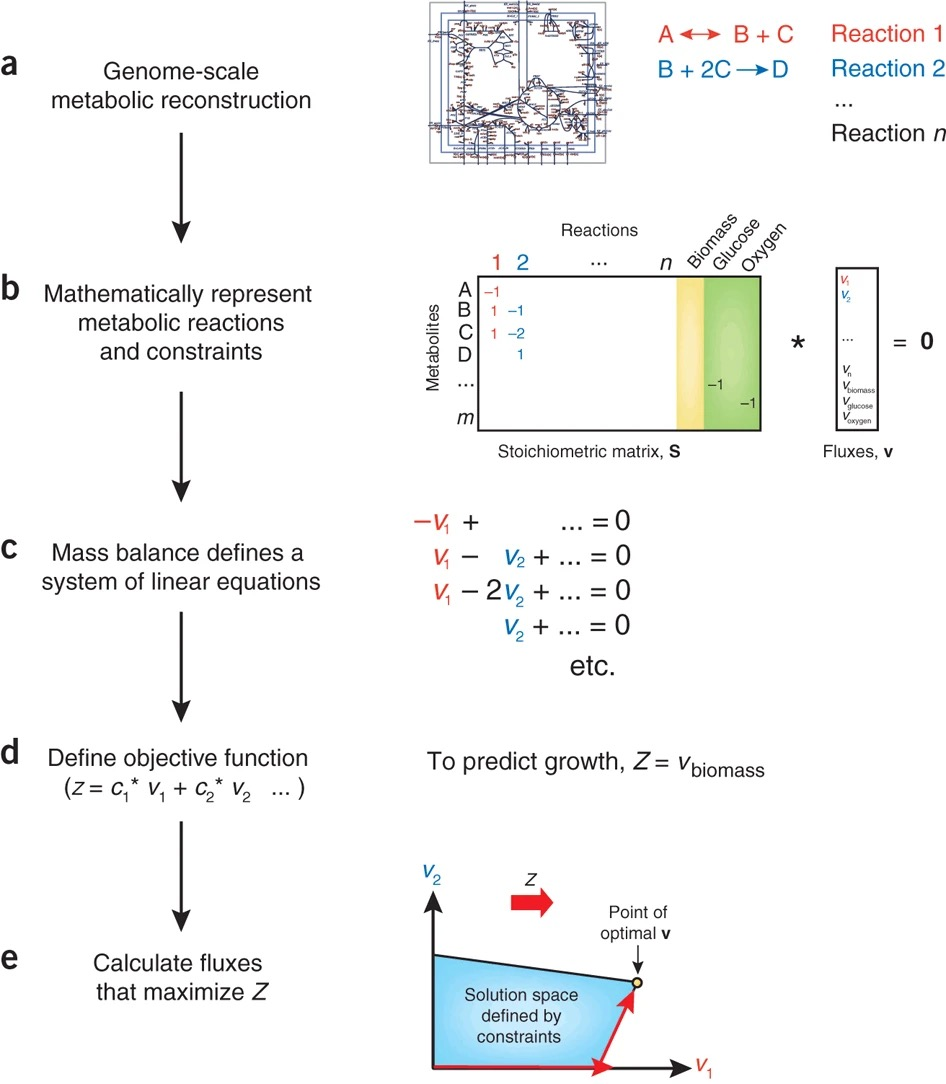
\includegraphics[width=0.9\linewidth]{fig/fba_workflow}
	\caption[Flowchart of constrained-based modelling]{Flowchart of constrained-based modelling. (a) Based on the genome of the organism, its metabolic network is reconstructed. (b) This network can be mathematically represented as a stoichiometric matrix S where each row stands for a metabolite and a column represents a reaction; each reactions has an associated flux value in the vector v. (c) Under the steady-state assumption, the matrix S and vector v form a system of linear equations. (d) Solving the equations required the definition of an objective function Z, which will be maximised during the optimisation step. (e) Linear programming is used to solve the linear equations and thereby find a flux distribution that maximises Z within the constrained solution space. Taken from \cite{orth_what_2010}.}
	\label{fig:fbaworkflow}
\end{figure}

\subsection{Reconstructing GEMs}
The basis for metabolic models forms an annotated genome, based on which, reactions and metabolites of the target organism can be inferred. Various tools have been developed to facilitate the reconstruction process. This process generally follows three steps: 
(i) Use databases and other prior knowledge to map the annotated genome to metabolic functions. 
(ii) Generate draft model. 
(iI) Curate the draft model.
A comprehensive review for tools employed in model reconstruction, quality control and curation can be found in \cite{tarzi_emerging_2024}.


Model reconstruction follows one of two approaches, or a combination of both. The first approach, known as 'top-down', begins with an existing network of biochemical reactions based on either genome-scale metabolic models that have already been reconstructed or a collection of all the reactions that have been identified in the organism of interest. This approach is typically faster and easier to automate, but lacks highly specific pathways and ideal accuracy. The second approach, called bottom-up, starts with known metabolic pathway stoichiometries and subsequently adds all known reactions and metabolites. This approach is much more time-consuming and labour-intensive, but it ensures very high accuracy and high quality models.
\\


A variety of tools can be employed to aid the model reconstruction. CarveMe (\cite{machado_fast_2018}) is one example of a tool that follows the top-down approach. Based on the entire bacterial metabolism in the BiGG database (\cite{king_bigg_2016}), it builds a universal model. All metabolites and reactions use BiGG identifiers. Additionally, each metabolite identifier ends with \_c, \_p or \_e according to its compartment (cytosol, periplasm or extracellular space).  According to the annotated genome of the target bacteria, the ‘carving’ process removes reactions and metabolites that are not predicted to occur in the organism. Depending on the gram-stain of the bacteria, it assigns a universal biomass function, which is a pseudoreaction that consists of all components required to produce new cell mass and the associated energy. CarveMe outputs the draft SBML model in .xml format that can be further analysed with COBRApy.

\subsubsection{Biomass in metabolic models}
\subsubsection{Biomass in metabolic models}
Fluxes are typically reported in $\text{mmol} \cdot \text{gDW}^{-1} \cdot \text{h}^{-1}$, where $\text{gDW}$ denotes gram dry weight of biomass and $\text{h}$ represents time in hours. The biomass metabolite within a model is a pseudo-metabolite that is usually defined by its precursors in the biomass reaction, rather than a single chemical compound. The molecular weight of the biomass of a metabolic model is typically normalised so that $1\text{ mmol}$ biomass corresponds to $1\text{ gDW}$, which is calculated by multiplying the coefficient of each metabolite of the biomass reaction with its molecular weight calculated from the formula, then dividing the overall sum of all the products by $1000$ \cite{lieven_memote_2020}. Therefore, the flux through the growth reaction can directly be interpreted as a growth rate in units of:
\[
\frac{\text{new biomass (gDW)}}{\text{existing biomass (gDW)} \cdot \text{h}}
\]
which yields $\text{h}^{-1}$ \cite{machado_fast_2018}. In other words: the growth rate $\mu$ is the instantaneous fractional rate at which biomass increases, i.e.\ $\frac{dX}{dt} = \mu \cdot X$, so at each timepoint, for a growth rate of $2\text{ h}^{-1}$, biomass is momentarily increasing at $2\text{ g}$ new biomass per $1\text{ g}$ existing biomass per hour. Integrating this relationship over an hour:
\[
X(t) = X_0 \cdot e^{\mu t}
\]
For $t = 1$ and $\mu = 2$:
\[
X(1) = X_0 \cdot e^{2} \approx X_0 \cdot 7.39
\]
\subsection{Quality assessment and curation of GEMs}
\cite{thiele_protocol_2010} defined the core principles of model reconstruction, network evaluation, refinement and curation, which remain central to the process today and guide the development of new automated approaches (Fig. \ref{fig:curation_workflow}). The quality of the models depends on the reconstruction approach taken and the quality of the underlying data. Quality is assessed and refined iteratively. Automatic algorithms evaluate model quality by detecting gaps and dead ends and by assessing consistency between the model and its annotation. A subsequent curation step then corrects and refines the model until it is consistent with experimental observations and fits community quality standards, to ensure an accurate representation of biological reality (Fig. \ref{fig:curation_workflow}).

\begin{figure}[h]
	\centering
	
\includegraphics[width=1\textwidth]{fig/curation_workflow_linear}
	\caption[Curation workflow]{Curation workflow. After draft model generation, several iterative steps are applied to refine, evaluate and improve the model. This schematic highlights key steps of the curation process established by \cite{thiele_protocol_2010})}
	\label{fig:curation_workflow}
\end{figure}


Manual quality control is very time and labour intensive and thus facilitated by various tools, amongst which are MACAW (\cite{moyer_macaw_2025}) and MEMOTE (\cite{lieven_memote_2020}). MEMOTE provides a comprehensive testing for consistency, annotation, biomass composition, energy metabolism, GPR rules, and network topology. Each test returns a score, all individual scores are then summed and weighted to an overall quality score. MACAW focuses on structural and functional checks, such as identifying duplicated, dead ends, and thermodynamically infeasible loops. The output of these tools and proposed steps in the \cite{thiele_protocol_2010} protocol guide the curation process. 
\subsection{Tools for community modelling}
Microbial communities are a fundamental unit in complex ecosystems, and deciphering their functionality, structure and other properties is of high interest across different disciplines. Thus many methods and tools have been developed to study microbial interactions. To analyse such interactions on a metabolic level, tools like COMMA (\cite{mirzaei_gem-based_2024}), MICOM (\cite{diener_micom_2020}), PyCoMo (\cite{predl_pycomo_2024}) or ReMIND (\cite{oftadeh_constraint-based_2024}) build community from taxon models following the steady-state approach. The tools differ in their required taxonomic information, analysis of microbial interactions, formulation of the objective function, as well as compartmentalisation strategy and are comprehensively reviewed in (\cite{tarzi_emerging_2024}). 
\subsubsection{MICOM} \label{sec:MICOM}
MICOM combines individual strain models into a unified community model with a shared medium compartment. Specifically, the extracellular compartment of every single-taxon input model is connected via an exchange reaction to a shared pool (\_m) through which community members interact. Exchange reactions from the shared medium \_m compartment to an individual's extracellular compartment \_e are either uptakes or secretions, depending on the direction of reaction. 

The community growth rate $\mu_c$ is calculated as the weighted sum of the individual growth rates $\mu_i$ of each organism $i$ and its relative abundances $a_i$. MICOM offers two different optimisation strategies: \texttt{optimise()}, which is simply a (p)FBA solution for the whole community, and \texttt{cooperative\_tradeoff()}, which optimises the objective function under user-provided abundance data and a trade-off approach between community and individual growth rate maximisation. This prevents the exclusion of strains known to be abundant for the sake of maximising the community growth rate. In practice, MICOM first maximises $\mu_c$, yielding the maximum community growth rate $\mu_c^{max}$. Then, the chosen trade-off $\alpha \in [0,1]$ sets the minimum fraction of $\mu_c^{max}$ that has to be achieved. Setting the trade-off to 0 optimises for individual growth, whereas a trade-off of 1 solves for maximal community growth. This sets up the quadratic minimisation problem following L2 regularisation: 

\begin{equation}
	\begin{aligned}
		&\text{minimise} & &\sum_{i} \mu_i^2 \\
		&\text{s.t.}     & &\mu_c \geq \alpha \mu_c^{\max} \\
		&                & &\text{and community constraints}
	\end{aligned}
\end{equation}
	
	
It favors balanced solutions with more equally distributed growth rate across community members, which is shown to yield more realistic growth rates (\cite{diener_micom_2020}). 

